%        File: WeeklyResearchReport_4_19_21.tex
%     Created: Mon Apr 19 08:00 AM 2021 E
% Last Change: Mon Apr 19 08:00 AM 2021 E
%
\documentclass[a4paper]{article}
\usepackage{mathtools}
\usepackage{verbatim}
\usepackage{graphicx}
\usepackage{tabularx}
\usepackage{pgfplots}
\usepackage{adjustbox}
\usepackage{booktabs}
\makeatletter
\let\latex@xfloat=\@xfloat
\def\@xfloat #1[#2]{%
    \latex@xfloat #1[#2]%
    \def\baselinestretch{1}
    \@normalsize\normalsize
    \normalsize
}
\makeatother
\usepackage{amsmath}
\usepackage{mathtools}
\usepackage{epigraph}
\usepackage{cancel}
\usepackage{xcolor}
\newcommand\Ccancel[2][black]{\renewcommand\CancelColor{\color{#1}}\cancel{#2}}
\usepackage{algorithm}
\usepackage{graphicx}
\usepackage[noend]{algpseudocode}
\usepackage{gnuplot-lua-tikz}
\usepackage[utf8]{inputenc}
\usepackage{pgfplots}
\usepackage{tabularx}
\DeclareUnicodeCharacter{2212}{−}
\usepgfplotslibrary{groupplots,dateplot}
\usetikzlibrary{patterns,shapes.arrows}
\pgfplotsset{compat=newest}
\begin{document}
\begin{titlepage}

    \title{
    Weekly Research Report}


    \author{ Jeffrey Severino \\
        University of Toledo \\
        Toledo, OH  43606 \\
    email: jseveri@rockets.utoledo.edu}


    \maketitle

\end{titlepage}
\section{Current Research Direction}
\section{Research Performed In the Past 24 hours}

\subsection{Current Validation Work}

A comparison was conducted for a hollow cylinder undergoing uniform flow with
acoustic liners along the outer duct perimeter. The azimuthal mode number, reduced 
frequency, mach number and duct liner admittance is reported below,
\begin{align*}
    m &= 2 \\
    k &= \frac{\omega r_T}{A_T} = -1 \\
    M_x &= 0.5 \\
    \eta_T &= 0.72 + 0.42i
\end{align*} 
\begin{figure}[h!]
    \centering
    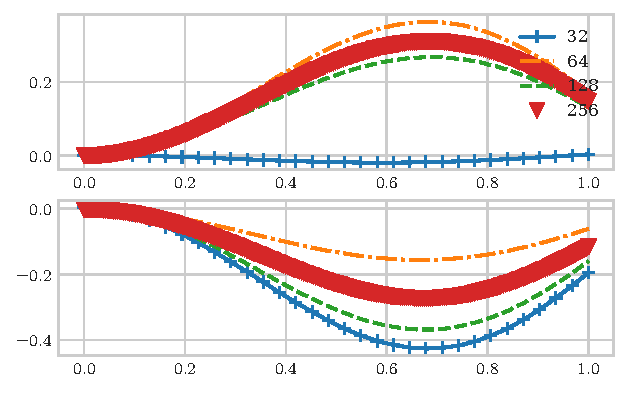
\includegraphics[width=\textwidth]{../../tex-outputs/egv1.pdf}
\end{figure}

\begin{figure}[h!]
    \centering
    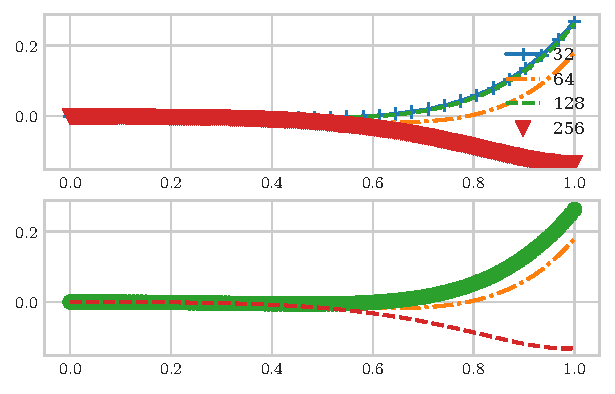
\includegraphics[width=\textwidth]{../../tex-outputs/egv2.pdf}
\end{figure}

\begin{figure}[h!]
    \centering
    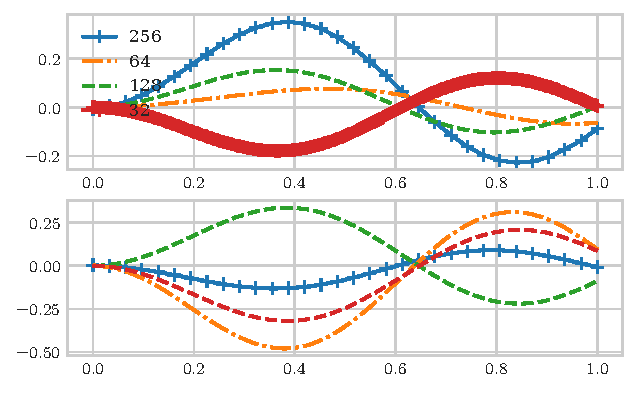
\includegraphics[width=\textwidth]{../../tex-outputs/egv3.pdf}
\end{figure}





I have reported the propagating modes for the first three axial wavenumbers at
four different grids

\section{Issues and Concerns}
The results look odd.. and do not seem to follow any particular trend. I have triple 
checked my data but the issue may not be apparent for these axial wavenumbers
\section{Planned Research}
See what the modes look like for all 9 wavenumbers in each case where we have 
cases to match
\end{document}


